\subsection{Câu lệnh if}
Câu lệnh if dùng để kiểm tra một điều kiện với đầu vào là một mệnh đề logic. Nếu điều kiện đúng sẽ thực hiện câu lệnh, nếu sai thì câu lệnh sẽ không được thực hiện.\par
Cấu trúc của câu lệnh if:\par
\texttt{if <condition>:}\par
\qquad \texttt{//conditional code}\par
\begin{figure}[h]
	\centering
	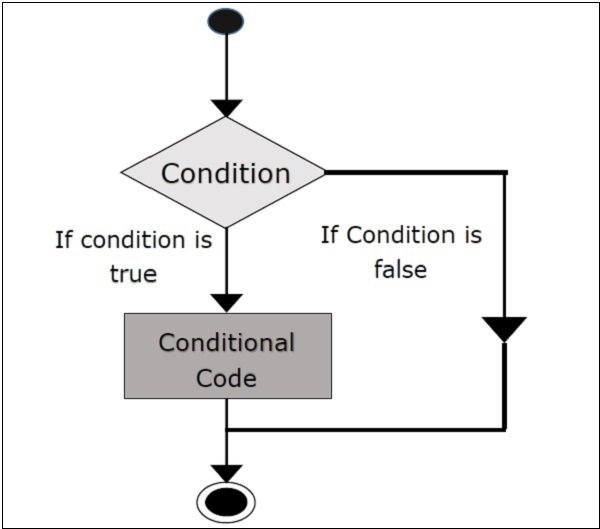
\includegraphics[width=0.7\linewidth]{img/if}
	\caption{Mô tả cách thức hoạt động của câu lệnh if}
\end{figure}
\newpage
\textbf{Ví dụ:} Chương trình nhập vào một số nguyên, nếu số đó là số chẵn thì in ra màn hình:\\
\rule{\linewidth}{0.2mm}\par
\begin{linenumbers}
	\texttt{number = \textcolor{red}{int}(\textcolor{blue}{input}("Type a number: "))}\par
	\texttt{\textcolor{red}{if} number \% 2 == 0:}\par
	\qquad \texttt{\textcolor{blue}{print}("\%d is an even number." \% number)}
\end{linenumbers}
\rule{\linewidth}{0.2mm}\par
\noindent
\resetlinenumber
Kết quả cho ra ở Console:\\
\rule{\linewidth}{0.2mm}\par
\begin{linenumbers}
	\texttt{Type a number: 12}\par
	\texttt{12 is an even number.}
\end{linenumbers}
\rule{\linewidth}{0.2mm}\par
\resetlinenumber
\newpage
\textbf{Ví dụ:}  Kiểm tra tuổi của sinh viên, nếu trên 17 là được chấp nhận:\\
\rule{\linewidth}{0.2mm}\par
\begin{linenumbers}
	\texttt{age = \textcolor{red}{int}(\textcolor{blue}{input}("Type your age: "))}\par
	\texttt{\textcolor{red}{if} age > 17: }\par
	\qquad \texttt{\textcolor{blue}{print}("Accepted!")}
\end{linenumbers}
\rule{\linewidth}{0.2mm}\par
\noindent
\resetlinenumber
Kết quả cho ra ở Console:\\
\rule{\linewidth}{0.2mm}\par
\begin{linenumbers}
	\texttt{Type your age: 16}\par
\end{linenumbers}
\rule{\linewidth}{0.2mm}\par
\resetlinenumber
\newpage